% !TEX program = pdflatex
% !TEX options = --shell-escape -synctex=1 -interaction=nonstopmode -file-line-error "%DOC%"
\documentclass[notitlepage]{article}
\usepackage{float}
\usepackage{verbatim}
\usepackage{amsmath}
\usepackage{listings}
\usepackage{bm}
\usepackage{graphicx}
\usepackage{booktabs}
\usepackage{color,xcolor}
\usepackage{enumerate}
\usepackage{minted}

\title{Poisson-FBMP Note}
\date{}

\definecolor{dkgreen}{rgb}{0,0.6,0}
\definecolor{gray}{rgb}{0.5,0.5,0.5}
\definecolor{mauve}{rgb}{0.58,0,0.82}
\lstset{
    language=python,
    basicstyle=\footnotesize,
    numbers=left,
    numberstyle=\tiny\color{gray},
    stepnumber=2,
    numbersep=5pt,
    backgroundcolor=\color{white},
    showspaces=false,
    showstringspaces=false,
    showtabs=false,
    frame=single,
    rulecolor=\color{black},
    tabsize=2,
    captionpos=b,
    breaklines=true,
    breakatwhitespace=false,
    title=\lstname,
    keywordstyle=\color{blue},
    commentstyle=\color{dkgreen},
    stringstyle=\color{mauve},
    escapeinside={\%*}{*)},
    morekeywords={*,...}
}

\begin{document}
\newcommand{\ud}{\mathrm{d}}

\maketitle

\section{P-FBMP only fitting}

\begin{lstlisting}
def optit0mu(t0, mu, n, xmmse_star, psy_star, c_star, la):
    ys = np.log(psy_star) - np.log(poisson.pmf(c_star, la)).sum(axis=1)
    ys = np.exp(ys - ys.max()) / np.sum(np.exp(ys - ys.max()))
    t0list = np.arange(t0 - 3 * Sigma, t0 + 3 * Sigma + 1e-6, 0.2)
    mulist = np.arange(max(1e-8, mu - 3 * np.sqrt(mu)), mu + 3 * np.sqrt(mu), 0.1)
    b_mu = [max(1e-8, mu - 5 * np.sqrt(mu)), mu + 5 * np.sqrt(mu)]
    tlist_pan = np.sort(np.unique(np.concatenate([np.unique(np.hstack(np.arange(1, window-1)[:, None] + np.arange(0, 1, 1 / n))), tlist])))
    As = np.zeros((len(xmmse_star), len(tlist_pan)))
    As[:, np.isin(tlist_pan, tlist)] = c_star
    tlist_edge = np.concatenate([[tlist_pan[0] - np.diff(tlist_pan)[0] / 2], (tlist_pan[1:] + tlist_pan[:-1]) / 2, [tlist_pan[-1] + np.diff(tlist_pan)[-1] / 2]])
    diff = np.diff(tlist_edge)
    assert As.sum() == c_star.sum()
    assert sum(np.sum(As, axis=0) > 0) > 0

    def likelihood(x):
        a = x[0] * wff.convolve_exp_norm(tlist_pan - x[1], Tau, Sigma) * diff + 1e-8 # use tlist_pan not tlist
        li = -special.logsumexp(np.log(poisson.pmf(As, a)).sum(axis=1), b=ys)
        return li

    likemu = np.array([likelihood([mulist[j], t0]) for j in range(len(mulist))])
    liket0 = np.array([likelihood([mu, t0list[j]]) for j in range(len(t0list))])
    mu, t0 = opti.fmin_l_bfgs_b(likelihood, x0=[mulist[likemu.argmin()], t0list[liket0.argmin()]], approx_grad=True, bounds=[b_mu, b_t0], maxfun=50000)[0]
    return mu, t0

truth = pelist[pelist['TriggerNo'] == ent[i]['TriggerNo']]

tlist = truth['HitPosInWindow'][truth['HitPosInWindow'] < right_wave - 1]
if len(tlist) == 1:
    tlist_edge = np.array([tlist[0] - 0.5, tlist[0] + 0.5])
else:
    tlist_edge = np.concatenate([[tlist[0] - np.diff(tlist)[0] / 2], (tlist[1:] + tlist[:-1]) / 2, [tlist[-1] + np.diff(tlist)[-1] / 2]])
t_auto = (np.arange(left_wave, right_wave) / wff.nshannon)[:, None] - tlist
A = p[2] * np.exp(-1 / 2 * (np.log((t_auto + np.abs(t_auto)) / p[0] / 2) / p[1]) ** 2)

t0_t = t0_truth[i]['T0']
mu_t = len(truth)
la = mu_t * np.array([integrate.quad(lambda t : wff.convolve_exp_norm(t - t0_t, Tau, Sigma), tlist_edge[i], tlist_edge[i+1])[0] for i in range(len(tlist))]) + 1e-8

c_star_truth = np.ones_like(tlist)
wav_ans = np.sum([np.where(pp > truth['HitPosInWindow'][j], wff.spe(pp - truth['HitPosInWindow'][j], tau=p[0], sigma=p[1], A=p[2]) * truth['Charge'][j] / gmu, 0) for j in range(len(truth))], axis=0)

mu, t0 = optit0mu(t0_t, mu_t, n, np.empty(len(la))[None, :], np.array([1]), c_star_truth[None, :], la)
\end{lstlisting}

Motivation: to validate fitting process

Progress: Use true \texttt{HitPosInWindow} as \texttt{tlist}, true \texttt{T0} as \texttt{t0\_t}, length of \texttt{HitPosInWindow} as \texttt{mu\_t}. Without FBMP RGS, directly \textbf{fit} $\mu$ and $t_0$. 

Result: fitting process is not related to bias of $\mu$. 

\begin{figure}[H]
    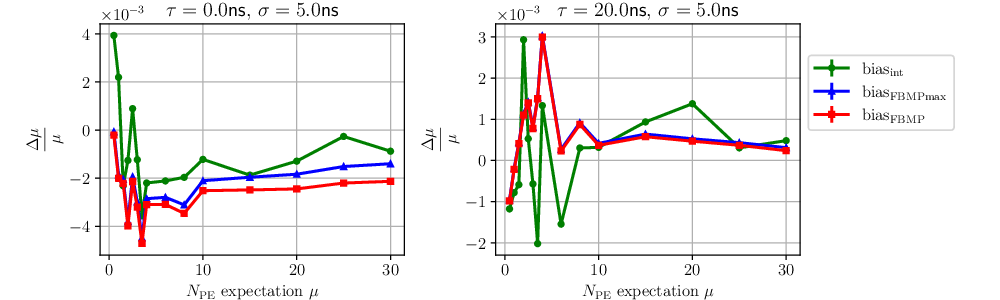
\includegraphics[width=\textwidth]{vs-biasmu-trufit.png}
\end{figure}

\section{P-FBMP with truth prior}

\begin{lstlisting}
tlist = truth['HitPosInWindow'][truth['HitPosInWindow'] < right_wave - 1]
if len(tlist) == 1:
    tlist_edge = np.array([tlist[0] - 0.5, tlist[0] + 0.5])
else:
    tlist_edge = np.concatenate([[tlist[0] - np.diff(tlist)[0] / 2], (tlist[1:] + tlist[:-1]) / 2, [tlist[-1] + np.diff(tlist)[-1] / 2]])
t_auto = (np.arange(left_wave, right_wave) / wff.nshannon)[:, None] - tlist
A = p[2] * np.exp(-1 / 2 * (np.log((t_auto + np.abs(t_auto)) / p[0] / 2) / p[1]) ** 2)
t0_t = t0_truth[i]['T0']
mu_t = len(truth)
factor = np.sqrt(np.diag(np.matmul(A.T, A)))
A = np.matmul(A, np.diag(1. / np.sqrt(np.diag(np.matmul(A.T, A)))))
la = mu_t * np.array([integrate.quad(lambda t : wff.convolve_exp_norm(t - t0_t, Tau, Sigma), tlist_edge[i], tlist_edge[i+1])[0] for i in range(len(tlist))]) + 1e-8
xmmse, xmmse_star, psy_star, nu_star, nu_star_bk, T_star, d_tot_i, d_max_i, num_i = wff.fbmpr_fxn_reduced(wave_r, A, la, spe_pre[cid]['std'] ** 2, (gsigma * factor / gmu) ** 2, factor, len(la), stop=5, truth=truth, i=i, left=left_wave, right=right_wave, tlist=tlist, gmu=gmu, para=p)
c_star = np.zeros_like(xmmse_star).astype(int)
for k in range(len(T_star)):
    t, c = np.unique(T_star[k][xmmse_star[k][T_star[k]] > 0], return_counts=True)
    c_star[k, t] = c
mu = np.average(c_star.sum(axis=1), weights=psy_star)
t0 = t0_t
\end{lstlisting}

Motivation: to prove prior used in FBMP is not the origin of $\mu$ bias. 

Progress: Use true \texttt{HitPosInWindow} as \texttt{tlist}, true \texttt{T0} as \texttt{t0\_t}, length of \texttt{HitPosInWindow} as \texttt{mu\_t}. \texttt{la} is vector of integral in each time bins. 

Result: prior used in FBMP is not the origin of $\mu$ bias. 

\begin{figure}[H]
    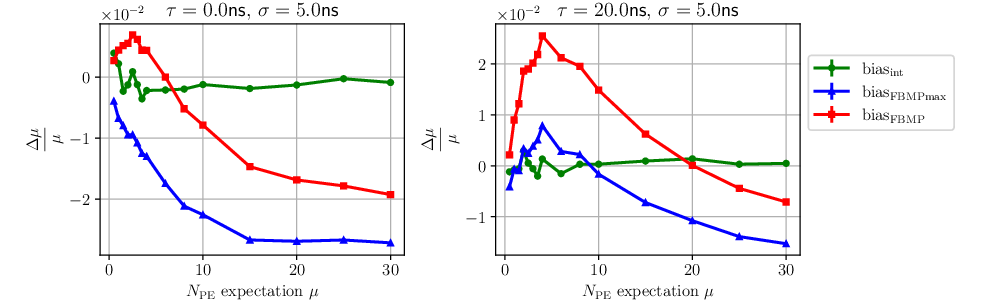
\includegraphics[width=\textwidth]{vs-biasmu-truprior.png}
\end{figure}

\end{document}